\chapter{Arquitetura}

A arquitetura foi pensada para ser implementada com o Docker e Docker Compose. Cada
programa que é executado é rodado em um serviço separado, portanto se o banco de dados,
por exemplo, tiver que ser reiniciado consigo usar o comando \texttt{docker compose down \&\& docker compose up -d}
para reiniciar apenas este container em específico.

\begin{figure}[ht]
    \begin{center}
    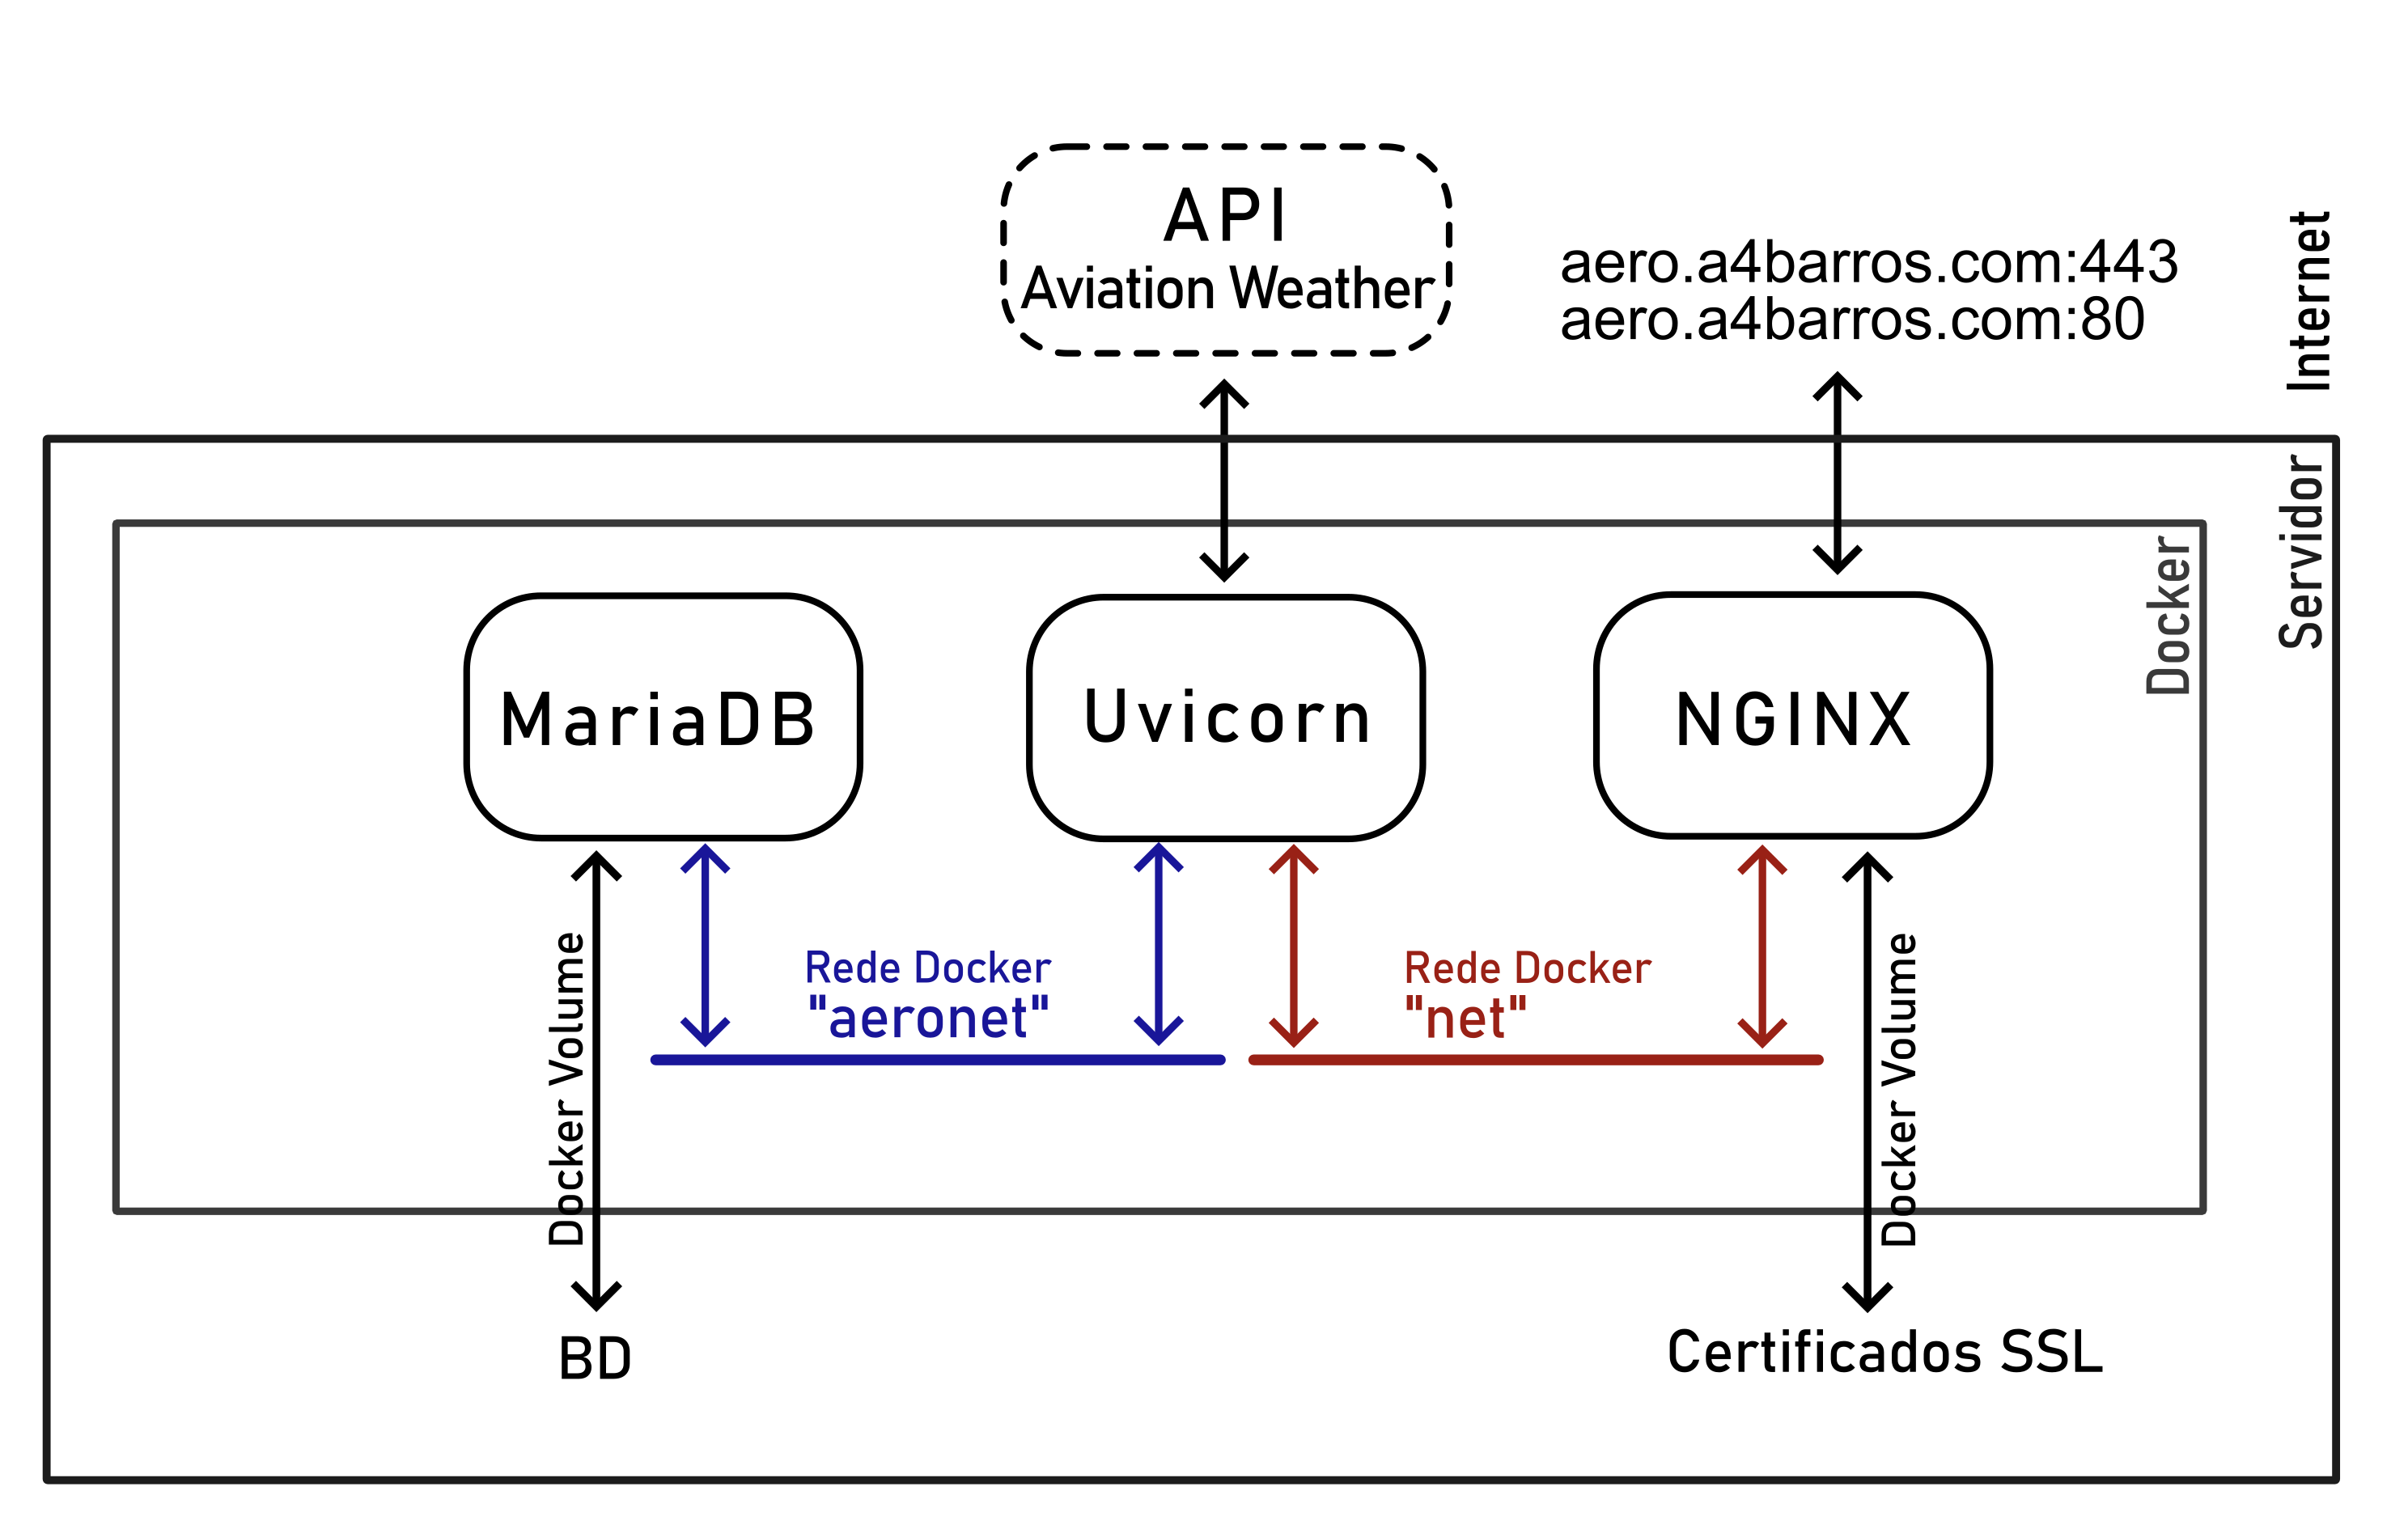
\includegraphics[width=\linewidth]{img/diagrama-arquitetura.png}
    \caption{Modelo de Arquitetura}
    \label{fig:arquitetura}
    \end{center}
\end{figure}

\section{Docker Network}
A porta 5000 do Uvicorn não estará disponível para todos os serviços. Por segurança, é usada a função de
"network". Observe no diagrama que a proxy NGINX compartilha com o Gunicorn a rede "net", para o NGINX,
o Uvicorn não pode ser acessado por \texttt{localhost:5000}, e sim por \texttt{http://aero:5000}, "aero"
sendo o nome do serviço no Docker Compose. Na máquina host e em containers que não tenham a rede
configurada para estas, não conseguem ver o Uvicorn.


\section{Docker Secrets}

Para aumentar a segurança de acesso ao banco, é usada a funcionalidade "secrets". Nela, no Docker Compose,
você informa um arquivo de texto no host onde estará uma senha, uma senha por arquivo. No mesmo Compose,
você informa quais serviços têm acesso a cada senha. Caso o serviço de banco de dados, por exemplo, tenha
acesso a senha db-password.txt, será feito um bind do arquivo db-password.txt no host para o "/run/secret/db-password.txt"
no guest.
Tanto os bancos como o servidor Gunicorn usam este método para terem acesso às senhas dos bancos.

\section{Serviços}

\subsection{MariaDB}
Este banco de dados relacional guarda toda a informação fixa sobre os aeródromos e as dinâmicas
como o METAR e TAF conforme explicado no capítulo de modelo de dados. É um banco tradicional
da indústria é extremamente confiável. Preferi usar ele, pois estou mais familiarizado com 
os comandos dele como \texttt{show tables} e \texttt{describe Aerodrome} do que os do PostgreSQL,
por exemplo, que seriam \texttt{\textbackslash dt} e \texttt{\textbackslash d+ Aerodrome}.

\section{FastAPI}

O site foi construído com a framework FastAPI. Tanto para desenvolvimento quanto para produção, 
é utilizado o servidor embutido do FastAPI, o Uvicorn. A configuração padrão funcionou bem ao
longo do tempo. Como explicado com mais detalhes do capítulo "Proposta", apesar do FastAPI ser
usado normalmente para a construção de APIs, ele pode retornar qualquer tipo de dado, inclusive
imagens, vídeos e páginas HTML. Para páginas HTML precisa ser informado no decorator que A
classe de resposta é "HTMLResponse".

\lstinputlisting[label=cod:plot, title={a}, caption={a}, language=Python]{code/html_resp.py}

\subsection{Proxy NGINX}
O NGINX realiza o SSL, dá suporte ao HTTP/2 e ao cabeçalho HTTP keep-alive. Quando
utilizava o Gunicorn, ele só tinha suporte ao primeiro, e a documentação do Gunicorn não
recomendava que ele estivesse diretamente ligado à Internet \cite{nginx-gunicorn}. O Uvicorn,
no momento em que este texto foi escrito, não suporta HTTP/2, mas suporta o keep-alive. No
entanto, como tenho outros projetos na mesma máquina, utilizo subdomínios. Todos os subdomínios
resolvem para a mesmo IP/máquina via "A RECORD", mas na configuração
do NGINX, o bloco de servidor com o hostname aero.a4barros.com é redirecionado para o
endereço interno "http://aero:5000".


\begin{figure}[ht]
    \begin{center}
    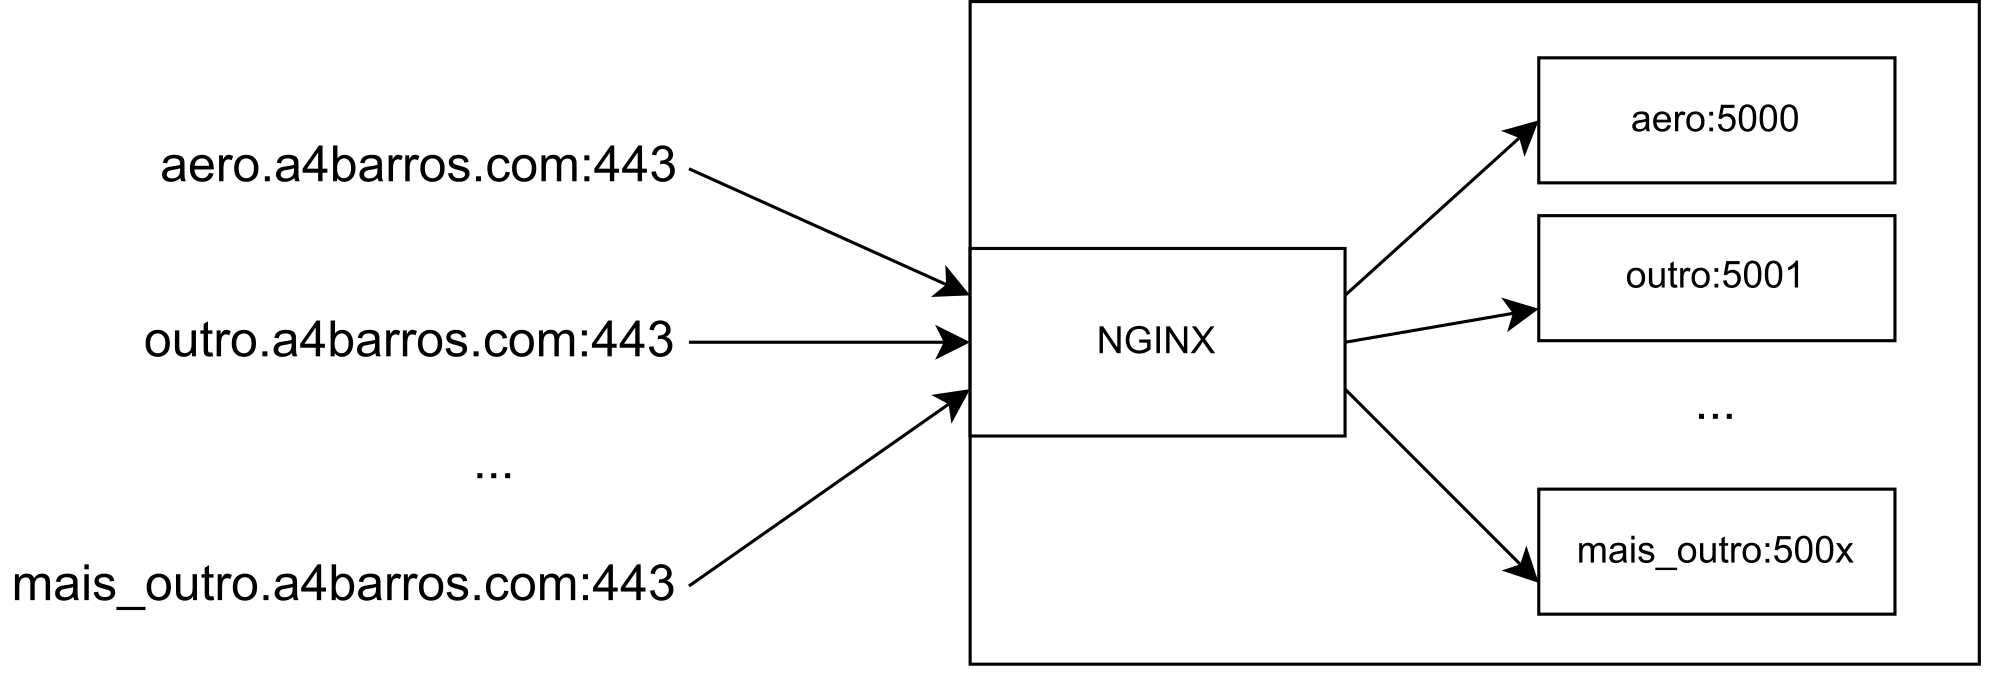
\includegraphics[width=400pt]{img/arquit.png}
    \caption{Diagrama do funcionamento de vários subdomínios resolvendo no mesmo IP. Com o NGINX funcionando como proxy.}
    \label{fig:sbrf-plot}
    \end{center}
\end{figure}

\section{Produção}
O site se encontra em produção no endereço https://aero.a4barros.com. Ele está hospedado em uma VPS
da Oracle Cloud Infrastructure com as seguintes características de hardware:

\begin{itemize}
    \item \textbf{CPU:} AMD EPYC 7551 (2 cores) @ 1.996GHz
    \item \textbf{RAM:} 1GB
    \item \textbf{Armazenamento:} 25GB
    \item \textbf{SO:} Ubuntu 22.04.4 LTS
\end{itemize}

\begin{figure}[ht]
    \begin{center}
    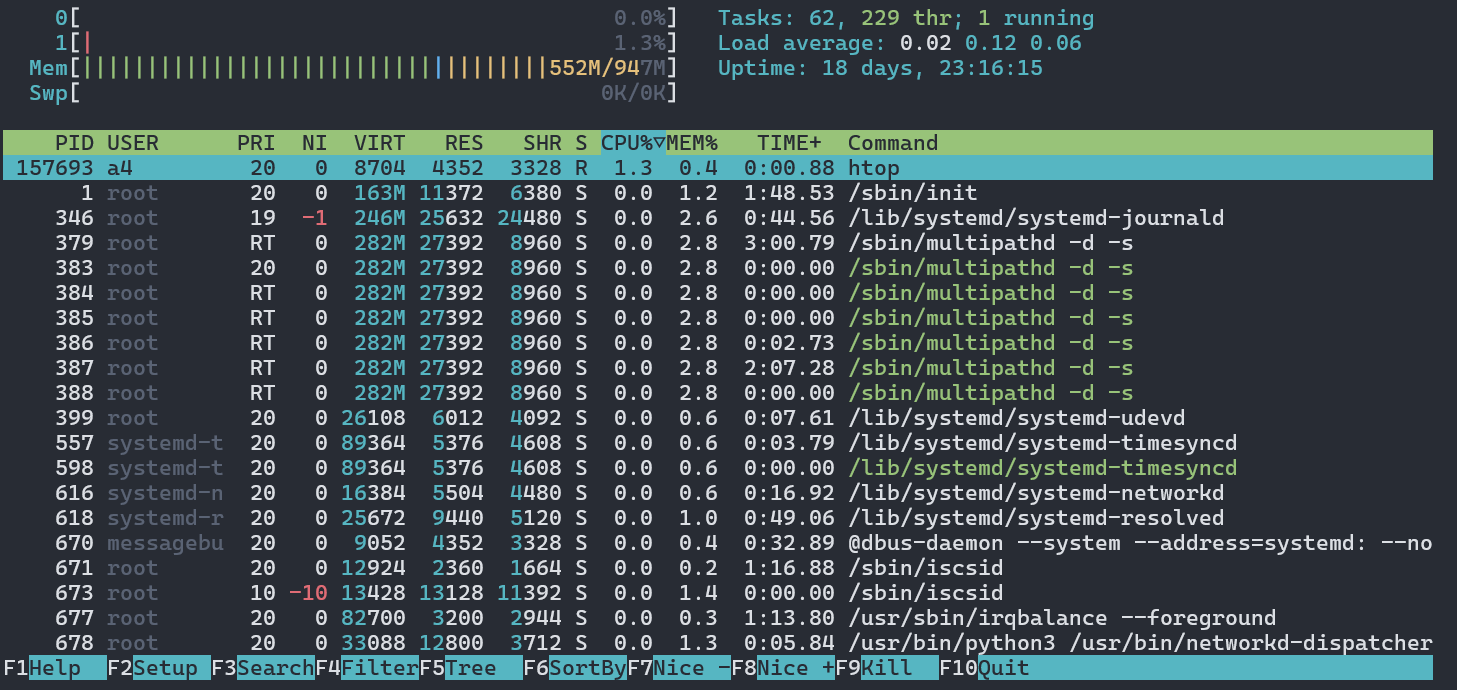
\includegraphics[width=400pt]{img/prod-idle.png}
    \caption{Uso do sistema em baixa demanda}
    \label{fig:prod-idle}
    \end{center}
\end{figure}

Mesmo com uma configuração bastante modesta, o sistema roda sete containers Docker, usando 
aproximadamente metade da memória primária (RAM) em idle.

\begin{figure}[ht]
    \begin{center}
    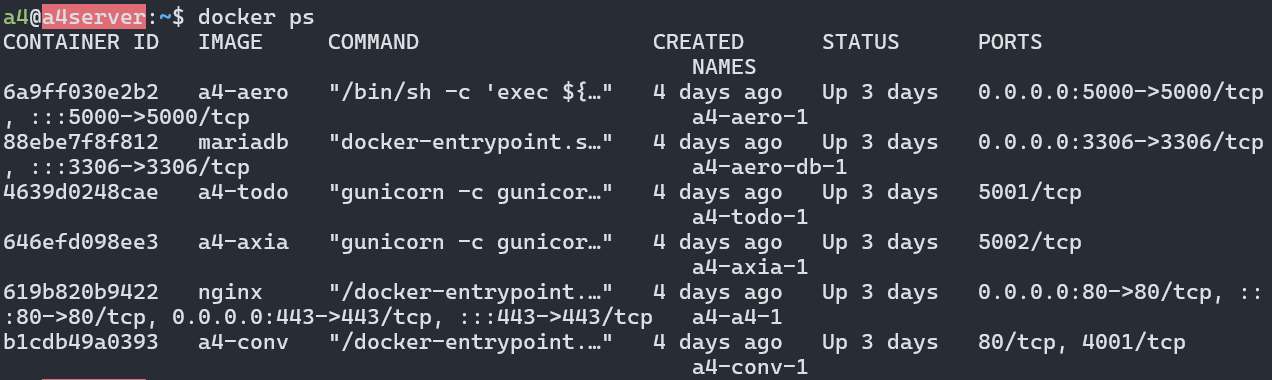
\includegraphics[width=400pt]{img/containers.png}
    \caption{Containers Docker em execução}
    \label{fig:containers}
    \end{center}
\end{figure}

\section{Operações Síncronas e Assíncronas}

Existem operações que ocorrem quando o usuário acessa uma página e outras que
ocorrem de tempos em tempos independentemente dos acessos (assíncronas). Fiz
esta separação para garantir que as APIs externas (METAR e TAF) sejam acessadas 
apenas quando
necessário sem que uma quantidade grande de acessos ao meu site sobrecarregue as estas APIs.

O desenho dos plots com dados históricos é uma operação que demora aproximadamente
3 segundos por aeródromo, então faço esta operação em background e deixo o 
arquivo .svg já pronto em uma pasta específica.

A seguir está descrito quando ocorrem estas operações assíncronas. Note que são
feitas com mais frequência que o necessário para se ter certeza que uma informação não
ficará muito tempo desatualizada caso ocorra algum atraso para atualização do METAR/TAF.

\begin{longtable}{|p{3cm}|p{4cm}|p{4cm}|}
    \caption{Operações assíncronas} \\
    \hline
    \textbf{Nome da função} & \textbf{Quando ocorre} & \textbf{Descrição}\\ \hline
    \endfirsthead
    \multicolumn{3}{c}%
    {{\tablename\ \thetable{} -- Continuação da página anterior}} \\
    \hline
    \textbf{Nome da função} & \textbf{Quando ocorre} & \textbf{Descrição}\\ \hline
    \endhead
    \hline \multicolumn{3}{|r|}{{Continua na próxima página}} \\ \hline
    \endfoot
    \hline
    \endlastfoot
        update\_metars
        & De vinte em vinte minutos
        & Normalmente um novo METAR é disponibilizado em cada hora, mas é possível ter um METAR a cada meia hora
        ou até menos. Para cada ICAO presente na tabela Aerodrome, cria-se um novo registro na tabela METAR
        com o novo METAR obtido caso este seja mais novo que o último presente no banco (é
        verificada a coluna updatedOn).
        \\ \hline

        update\_tafs
        & De três em três horas
        & O mesmo só que para os TAFs. Os TAFs são atualizados com menos frequência que os METARs, Normalmente nos
        horários 00:00, 06:00, 12:00 e 18:00 UTC.
        \\ \hline

        update\_images
        & De vinte em vinte minutos
        & Criação dos plots. Obviamente precisa ter a mesma frequência da atualização de METAR.
        \\ \hline

\end{longtable}

\section{Diagrama de sequência}

\begin{figure}[ht]
    \begin{center}
    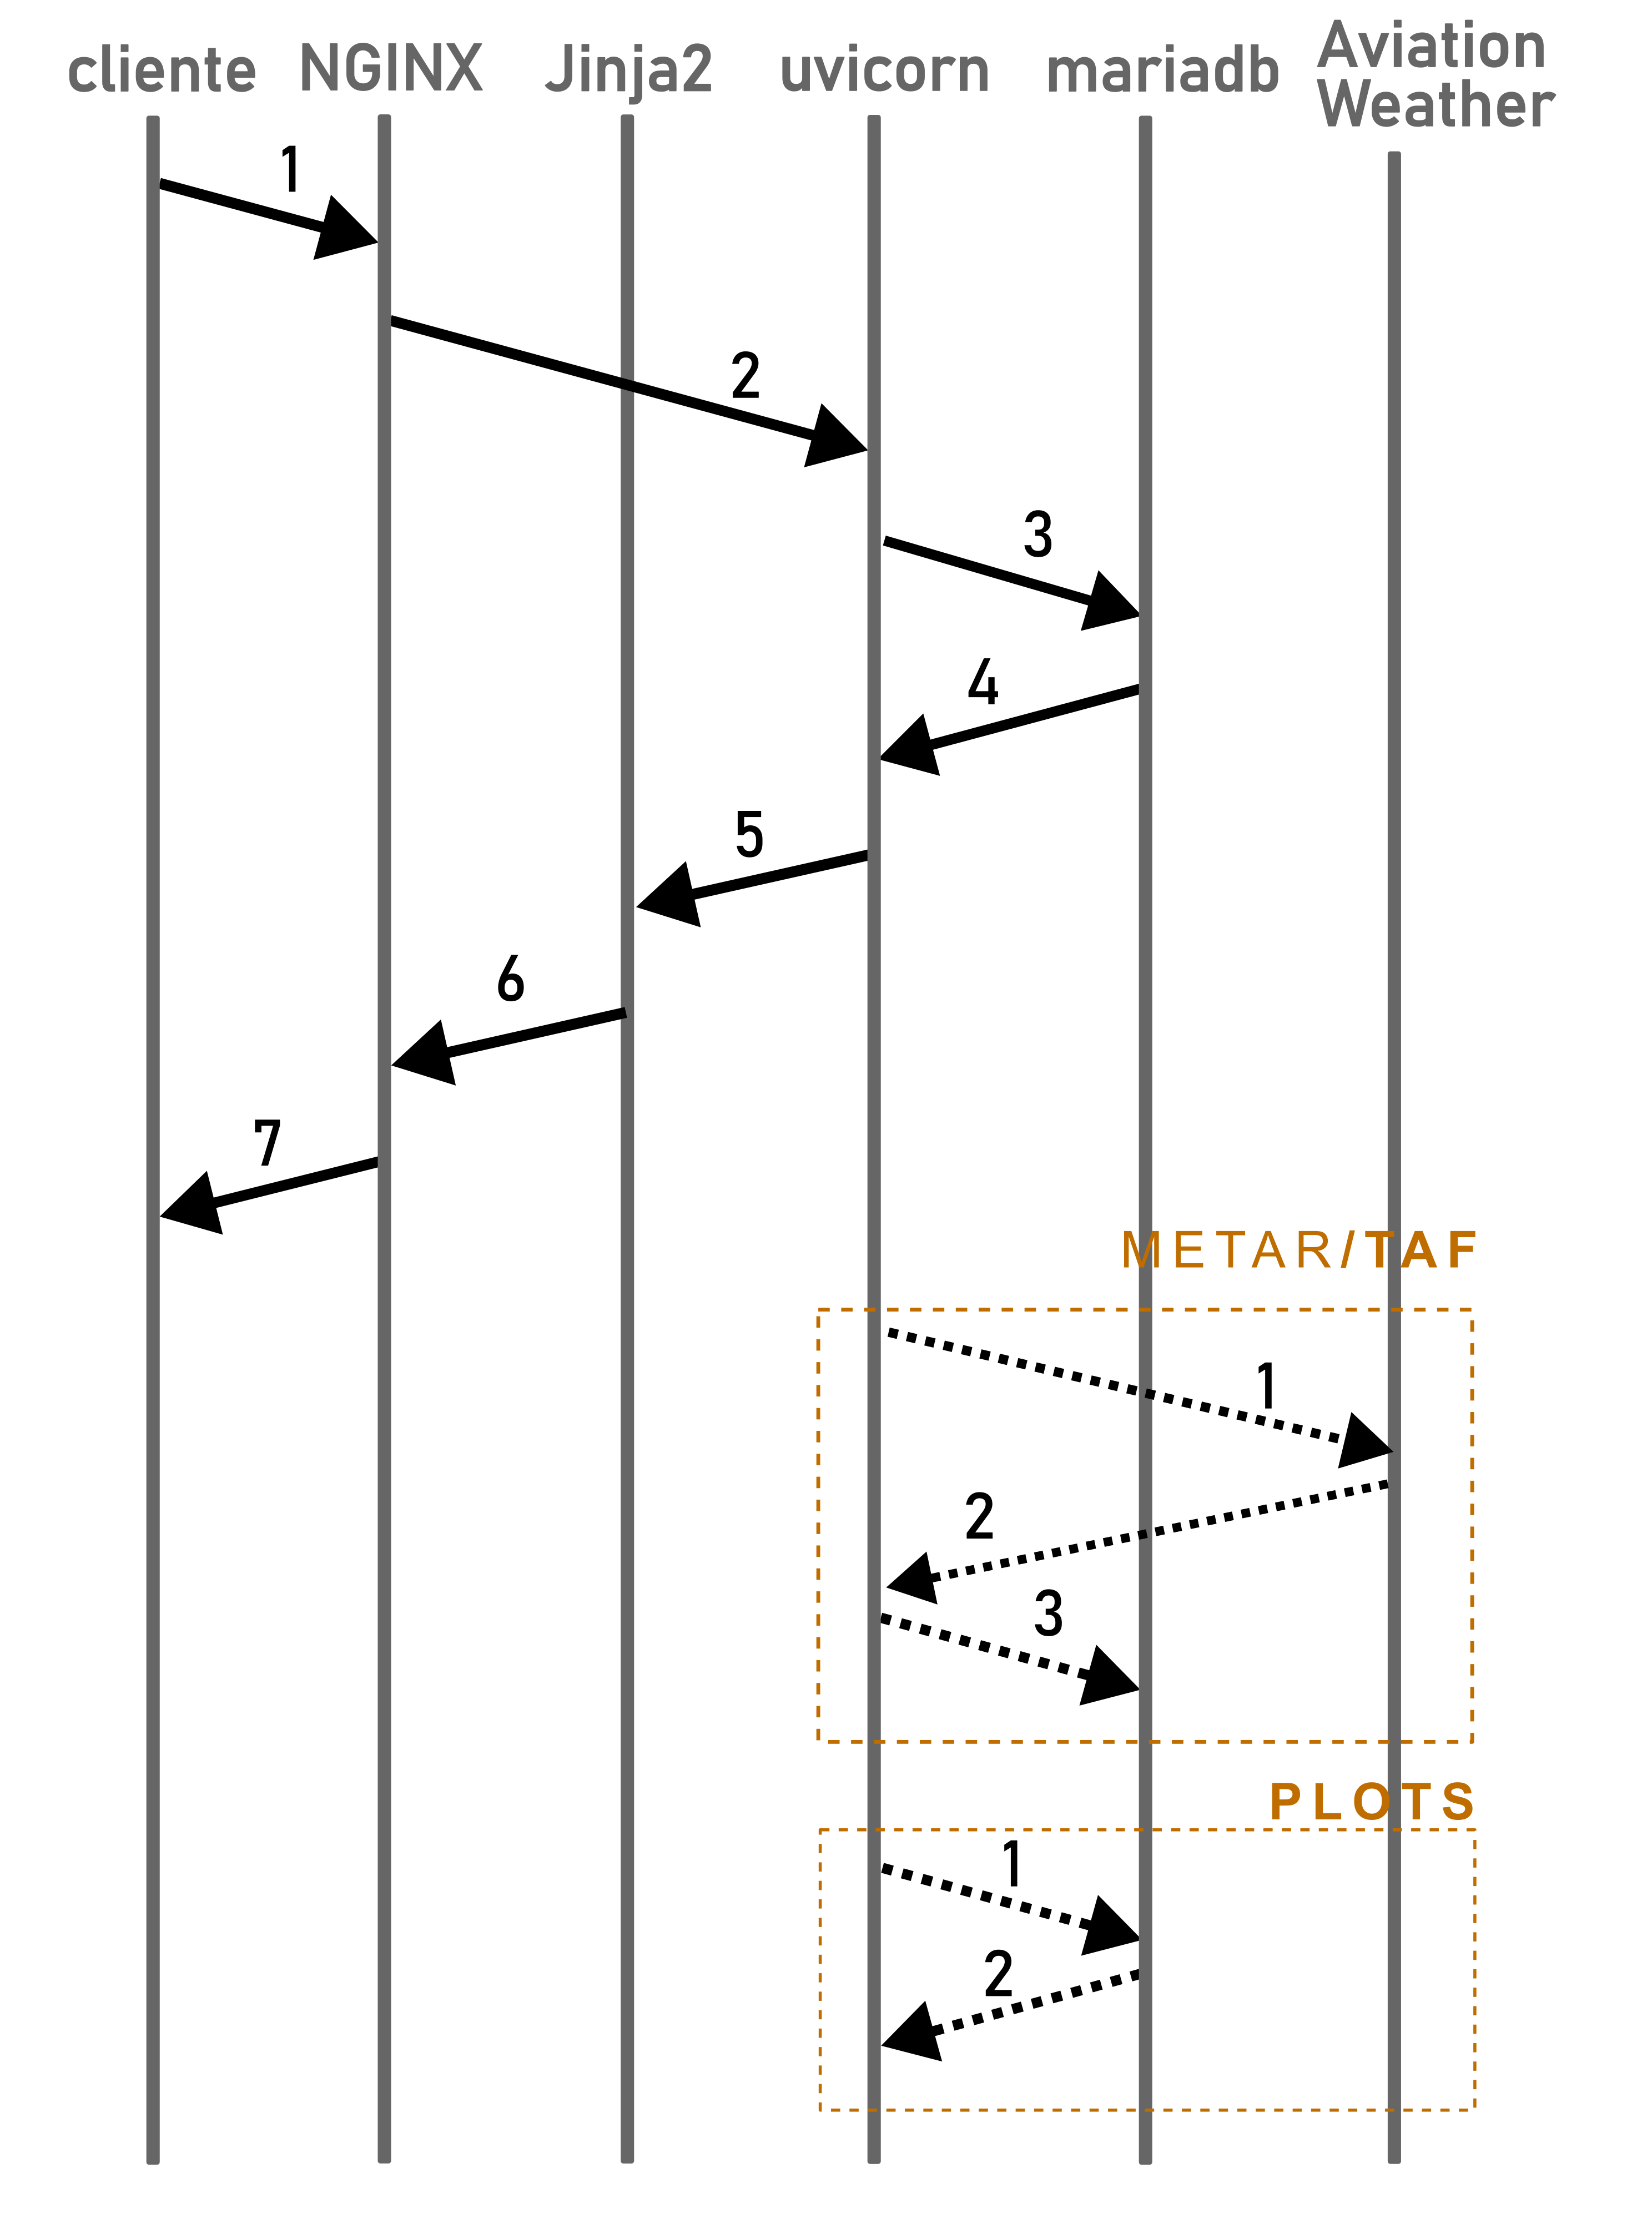
\includegraphics[width=0.5\linewidth]{img/diagrama-tempo.png}
    \caption{Diagrama de sequência}
    \label{fig:tempo}
    \end{center}
\end{figure}

\begin{enumerate}
\item O usuário realiza uma requisição para a rota raiz, "/info/\{icao\}", "/taf/\{icao\}"
ou "/history/\{icao\}"
\item Um servidor NGINX funcionando como proxy realiza o limite de requisições por segundo
e bloqueia user-agents que aparentam serem robôs. Caso a requisição passe pelo filtro, é
realizado um proxy-pass para o servidor Uvicorn.
\item Para a rota raiz, é feito um SELECT no banco para pegar informações de todos os
aeroportos. Na rota "/info/\{icao\}", é feito um SELECT-WHERE na tabela METAR, ILS, Communication, Runway...
Na rota "/taf/\{icao\}" é feito o mesmo, mas na tabela TAF. Para a rota "/history/\{icao\}"
não há acesso ao banco.
A ORM é usada para isto, portanto os comandos SQL não aparecem diretamente no código.
\item O banco de dados responde à requisição.
\item O servidor envia as informações necessárias ao Jinja2 para a geração da página.
\item A página HTML é gerada.
\item O usuário recebe esta página.
\end{enumerate}

No momento de atualizar os METARs e TAFs os seguintes passos acontecem.

\begin{enumerate}
\item É feita uma requisição para a API do Aviation Weather pedindo o METAR para os aeroportos
cadastrados esta API permite informar uma lista de ICAOs separados por vírgula.
O mesmo é feito com outra rota desta API que responde com os TAFs.
\item A API responde.
\item Os METARs e TAFs atualizados são gravados no banco.
\end{enumerate}

Para gerar as plotagens com informações históricas os seguintes passos acontecem.
\begin{enumerate}
    \item É feito um query para o banco pedir os 10 últimos METARs de cada aeródromo.
    \item O banco responde. A biblioteca matplotlib é usada para criar os plots que são salvo como SVGs 
    no path /static/plots.
\end{enumerate}